\section{印度佛教史}

\subsection{种性制度}
\begin{itemize}
  \item 婆羅門:祭司
  \item 剎帝利:武士
  \item 吠舍: 农工商业
  \item 首陀羅: 奴隶
\end{itemize}

\subsection{六派哲學}
產生於史詩時期之末,與佛教初期階段相近的婆羅門教哲學\footnote{木村泰賢$\cdot$《原始佛教思想論》}。
\begin{itemize}
  \item 尼夜耶派(The Nyāya School)。
  \item 僧佉耶派(The Sāṃkhya School)即數論派。
  \item 毘舍迦派(The Vaiśeṣika School)即勝論派。
  \item 瑜伽派(The Yoga School)。
  \item 弭曼差派(The Mīmāṃsā School)。
  \item 吠檀多派(The Vedānta School)。
\end{itemize}

\subsection{奧義書}
\begin{itemize}
  \item 業說,在《古奧義書》本為不公開的密教,到佛世則成為各教派所公認的思想
  \item 輪迴說,在梵書時代已萌芽,完成而為一般所承認,則自奧義書時代始
  \item 解脫說,乃為《奧義書》的最終目的
\end{itemize}

\subsection{六師外道}
記載常見於声闻經律\footnote{《長阿含經》第二十七經《沙門果經》}
\begin{itemize}
  \item 不蘭迦葉(Pūraṇa-Kāssapa):為倫理的懷疑者,否定善惡之業有其相應之根,故倡無作用論。
  \item 末伽梨瞿舍利(Makkhali Gosāla):此為邪命外道之祖,倡無因而有論。乃是耆那教的一派,在佛世極有勢力,除了耆那教,他是其餘五師中最盛大者。
  \item 阿耆多翅舍欽婆羅(Ajita Keśakambala):否定靈魂之說,倡唯物論,以快樂為人生之目的,排斥一切嚴肅的倫理觀念,此亦即是順世外道。
  \item 婆浮陀伽旃那(Pakudha Kaccāyana):主張心物永不消滅,倡世間常存論。
  \item 散若夷毘羅梨沸(Sañjaya Belaṭṭhiputta):為詭辯派或捕鰻論者,舍利弗(Śāriputra)及目犍連(Mahāmaudgalyāyana),即是此派出身而皈信佛教的。
  \item 尼乾陀若提子(Nigaṇṭha-Nātaputta):這就是耆那教之始祖摩訶毘盧(Mahā-vira),他出世稍早於釋尊,也是王子出身。此派以命(Jīva)及非命之(Ājīva)之二元論而說明一切,故也是否定有上帝造物觀念的無神論者。其實踐方面,則以極端的苦行及嚴守不殺生為特色。
\end{itemize}

\subsection{六十二見}
兩說及十類\footnote{《長阿含經》卷一四第二十一經《梵動經》}
\begin{itemize}
  \item 說過去世,或稱本劫本見者,五類十八見:
    \begin{itemize}
      \item 世間常住論,即是常見論,四種。
      \item 世間半常半無常論,四種。
      \item 世間有邊無邊論,四種。
      \item 異問異答論,即是詭辯派、捕鰻論、不死矯亂論,四種。
      \item 無因而有論,即是無因論,二種。
    \end{itemize}
  \item 說未來世,或稱末劫末見者,五類四十四見:
    \begin{itemize}
      \item 世間有想論,十六種。
      \item 世間無想論,八種。
      \item 世間非有想非無想論,八種。
      \item 眾生斷滅無餘論,即是斷見論,七種。
      \item 現法涅槃論,即無論在何種狀態,處於現世的即為最高的境界,五種。
    \end{itemize}
\end{itemize}

\subsection{家谱}
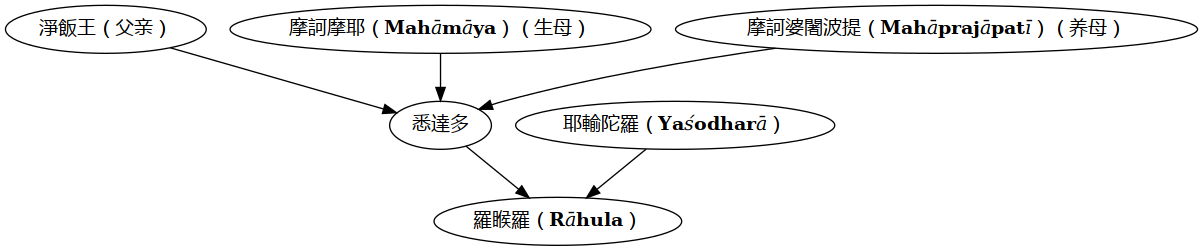
\includegraphics[width=\textwidth]{释家/images/释尊家谱.png}

\subsection{修道}
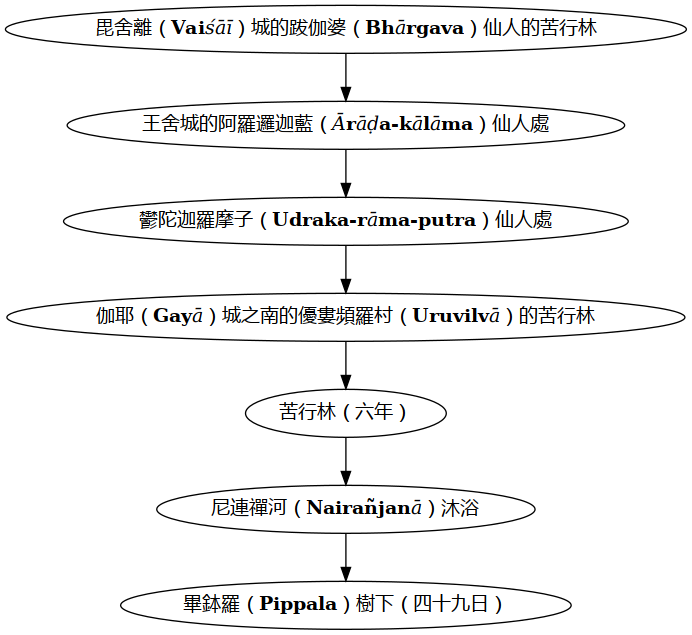
\includegraphics[width=\textwidth]{释家/images/释尊修行地图.png}

\subsection{四七日}
\begin{enumerate}
  \item 在菩提(Bodhivṛkṣa)樹下。就是那棵畢鉢羅樹之下,因佛在此樹下成道,而被稱為菩提樹
  \item 在阿踰波羅(Ajapāla)樹下。此期有魔王波旬(Māra-pāpīmān)來請佛入滅而未果。
  \item 在目真鄰陀(Mucilinda)樹下,遇暴風雨,目真鄰陀龍見之而即以己身護佛。此龍即受皈依,乃為傍生中的第一弟子。
  \item 在羅闍耶恆那(Rājāvatana)樹下。有二商主,一名提謂,一名婆梨迦,道經佛處,以麨蜜供佛,並皈依佛、法而去。此二人乃為最早的優婆塞(Upāsaka 親近而奉事三寶的淨信男)
\end{enumerate}

\subsection{轉法輪}
\begin{enumerate}
  \item 婆羅奈斯(Vārāṇiasī)城的鹿野苑\footnote{度五比丘: 阿若憍陳如(Ājñāta-Kauṇḍinỵa)、跋提(Bhadrika)、婆波(Vāṣpa)、摩訶男(Mahānāma)阿說示(Aśvajit)} 
\end{enumerate}
